\chapter{扰动场协同优化}

\section{协同模拟中的磁谱计算简化理论}
FLT 在最外闭合磁面的水平方向外平移 10 mm, FLT 会从下沿进入强场侧,为避免这种情况,向外平移 15 mm 余。
% \begin{figure}[t]
%   \centering

%   \subcaptionbox{基于磁力线追踪计算得到的螺旋电流丝轨迹,五条分别螺旋电流丝起点分别取为五排低杂波天线的中间位置正对着的闭合磁面外 10 mm 以内。}{%
%     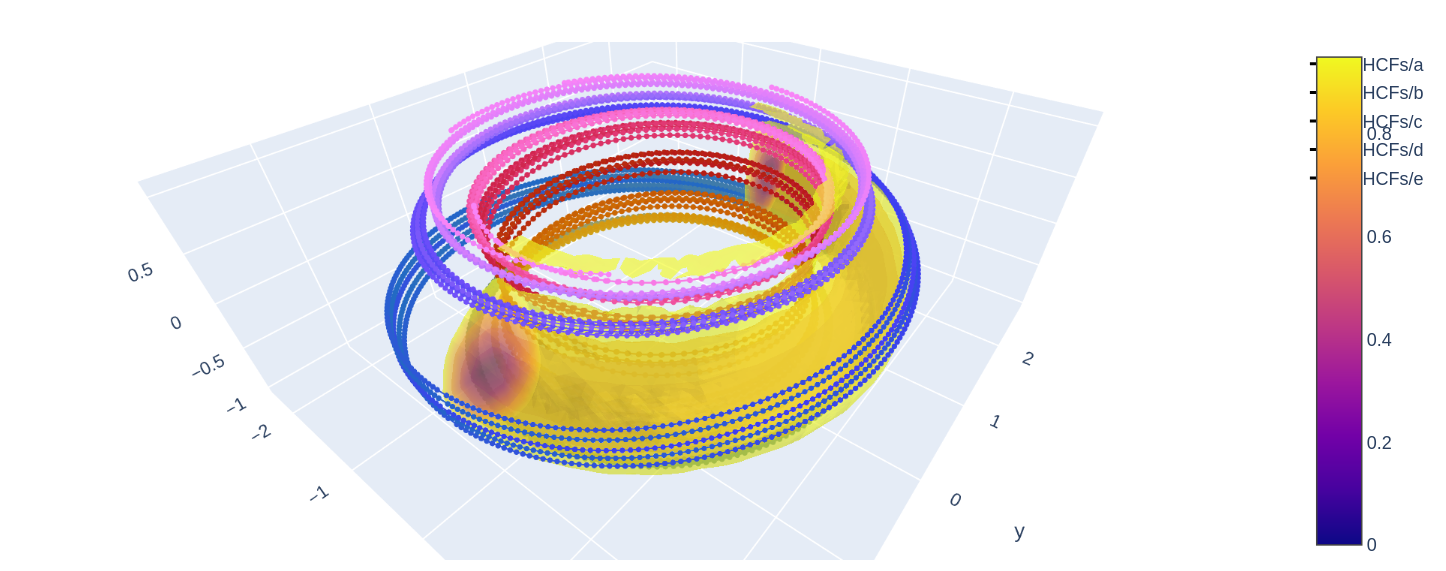
\includegraphics[width=0.47\columnwidth,keepaspectratio]{73999_030400ms_improved/hcfs_east.png}
%   }\hfill
%   \subcaptionbox{\east 上 RMP 线圈(低 n 线圈)、高 m 线圈及在闭合磁面外 15 mm 余处开始延伸的螺旋电流丝结构图。}{%
%   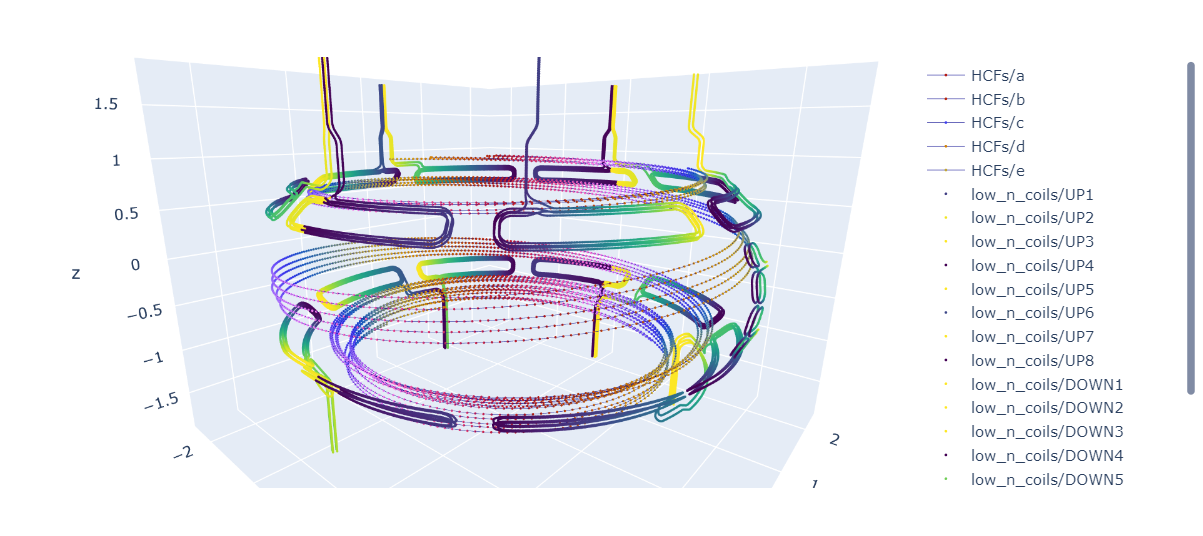
\includegraphics[width=0.47\columnwidth,keepaspectratio]{visual_coilsys.png}
% }
% \end{figure}

  高 m 线圈在 $\varphi$ 正方向上进行移动 $\Delta \varphi$,相当于$\tilde{b}_{m n}^{1}(s)$乘因子 $e^{-i\left(n \Delta\varphi \right )}$。

  下表罗列除了线圈电流幅值、相位及线圈位置等可调参数的可选空间。
  螺旋电流丝的电流强度和位置实验上不太好控制,暂时将其作为给定量,由其他线圈配合它。

  
\begin{table}[htb]
  \centering
  \caption{扰动场可调参量}
  \label{tab:east_parameter}
  \begin{tabularx}{\linewidth}{lXX}
      \toprule[1.5pt]
      变量 & 备注 & 可选区域 \\
      \midrule[1pt]
      $I_{amp~\text{UP}}$ & RMP 线圈上沿电流幅值 & $[-10 \text{kAt}, 10 \text{kAt}]$\\ 
      $I_{amp~\text{DOWN}}$ & RMP 线圈下沿电流幅值 & $[-10 \text{kAt}, 10 \text{kAt}]$\\ 
      $I_{amp~\text{high m, UP}}$ & 高 $m$ 线圈上沿电流幅值 & $[-10 \text{kAt}, 10 \text{kAt}]$\\
      $I_{amp~\text{high m, DOWN}}$ & 高 $m$ 线圈下沿电流幅值 & $[-10 \text{kAt}, 10 \text{kAt}]$\\
      $\Phi_{UP}$ & RMP 线圈上沿电流相位 & $[-\pi, \pi]$\\
      $\Phi_{DOWN}$ & RMP 线圈下沿电流相位 & $[-\pi, \pi]$\\
      $\phi_{\text{high m}}$ & 高 m 线圈环向分布角 & $[-\pi, \pi]$\\
      \bottomrule[1.5pt]
  \end{tabularx}
\end{table}
  
傅里叶变换的线性性、平移性大大减少了计算磁谱的成本。

  \begin{itemize}
    \item 线性性:线圈强度的变化,利用傅里叶变换的线性性减少计算量。
    \item 平移性:高 m 线圈的角度是指其自身物理位置在柱坐标系统沿中心轴进行环向上的旋转的角度,在 $(\theta^*, \varphi)$ 上沿着 $\varphi$ 平移 $\Delta\varphi$,利用傅里叶变换的平移性质,相当于$\tilde{b}_{m n}^{1}(s)$乘因子 $e^{-i\left(n \Delta\varphi \right )}$,。
    $$\Delta\varphi \Rightarrow e^{-i\left(n \Delta\varphi \right )}$$ 类似的,如果在极向角度上改变 $\Delta\theta^*$,则可以乘因子 $e^{-i\left(n \Delta\theta^* \right )}$。
  \end{itemize}  
  


\subsection{优化函数}

    
    这是偏工程方面的优化问题,目标函数有两个条件。一个是尽可能地生成强的边界随机场,这一方面我们用 Chirikov 参数来刻画;另一方面是希望新经典环向粘滞的影响尽可能地小,我们下面给出下面的评估标准。
    
  品质因子定义 (figure of merit, FoM),
  
  \begin{equation}
    FoM=\left[\frac{\langle\sigma\rangle_{s_{1}<s<s_{2}}^{4}}{\left\langle\sum_{m, n(n \neq 0)}\left[b_{m n}^{r}\right]^{2}\right\rangle_{s_{3}<s<s_{4}}}\right]
  \end{equation}
  
\begin{equation}
  b^r = \frac{\vect{B}\cdot\vect{n}}{B_0} = \frac{\vect{B}\cdot \nabla s}{B_0 |\nabla s|}
\end{equation}

我们同样对 $b^r$ 做类似 $\tilde{b}^1$ 的 Fourier 变换

\begin{equation}
  b_{m n}^{r}(s) \equiv \int_{\varphi=0}^{2 \pi} \int_{\theta^{*}=0}^{2 \pi} b^{r}\left(s, \theta^{*}, \varphi\right) e^{-i\left(m \theta^{*}+n \varphi\right)} \frac{d \theta^{*}}{2 \pi} \frac{d \varphi}{2 \pi}
\end{equation}

\begin{equation}
  b^{r}\left(s, \theta^{*}, \varphi\right)=\sum_{m, n=-\infty}^{\infty} b_{m n}^{r}(s) e^{i\left(m \theta^{*}+n \varphi\right)}
\end{equation}

  
其中分母是 $b^r$ 磁谱中分量平方的加和,用它来定性刻画新经典环向粘滞(Neoclassical Toroidal Viscosity, NTV)影响大小。当托卡马克的环向对称性被打破时,会有额外的力矩作用在等离子体上,从而形成共振的环向旋转频率,这被称为新经典粘滞效应。

当只考虑基频分量引起的磁岛时时,$\sigma\propto \sqrt{I_{coil}}$,Chirikov 参数与扰动场幅值成正比,而$b^r_{mn}\propto I_{coil}$,故而 Chirikov 参数取四次幂作为分子,从而扰动场的幅度变化不会影响该品质因子。
% 香蕉粒子在等离子体中以香蕉状轨迹往复运动导致的额外的粘性。


% 而关于

% $\tilde{b}_{r e s}^{1}$ The expression that we use for the physical effective radial RMPs is:
% \[
% b_{r e s}^{r} \equiv \frac{\tilde{b}_{r e s}^{1}}{R_{0}\langle\sqrt{g^{11}}\rangle_{\theta^{*}}}
% \]
% where the brackets represent an averaging over $\theta^{*}:\langle\sqrt{g^{11}}\rangle_{\theta^{*}} \equiv \int_{\theta^{*}=0}^{2 \pi} \sqrt{g^{11} \frac{d \theta^{*}}{2 \pi}} .$ 


  % \begin{enumerate}
  %   \item 在边界共振分量较大为好,越在边界产生的共振分量越重要,积分权重与到有理面共振线的距离成反比 $d=dist(point(n,m),q(\Psi_{pol})n)\downarrow, \rho(m,n,q) \uparrow$。
  %   \item 减去或除去芯部有理面的共振分量,减弱 2/1, 3/1 有理面存在的不稳定性反馈。。
  % \end{enumerate}
    
  % \begin{equation}
  %   \int_{\Psi_{pol}>0.87} \sum_{m,n} \rho(m,n,q) |B_{mn}^r| S(\Psi_{pol})d\Psi_{pol} - \sum_{internal~\Psi_{pol}} \sum_{m,n} \rho(m,n,q) |B_{mn}^r|
  % \end{equation}
  
  % 确定了优化函数后通过共轭梯度法找到一个较优解,或者算力允许的话画等位图。
  
    
  % 取磁面坐标$(s=\Psi^{1/2}_{pol},\theta^*,\varphi)$,


    
  
    




\section{扰动场协同模拟结果}
在协同模拟实验中,各扰动场在对应的场源为 \SI{1}{\kilo\ampere t} 时的扰动场被保存为场数据文件。标记各扰动场源正方向,\textit{(1) RMP 线圈 / 低 n 线圈} 产生的 $B^1$ 在作用的核心区为正即为正  \textit{(2) 高 m 线圈} 确定主要工作模式 $B^1$ 从上至下是 -,+,-,+ 分布,次要工作模式是 -,+,-; \textit{(3) 螺旋电流丝} FLT 电流沿磁场方向即为正方向

\subsection{三者扰动场共同作用}
  
  当首次进行实验时使三种扰动场同时加入到计算中中发现的一些问题。

  
     对于单零位型,上下两侧扰动场线圈产生的扰动场大小明显不同,使得电流相对大小参与到优化中更有必要。

     近期磁谱优化的试验发现,磁谱 $\tilde{b}^1_{mn}$ 的脊线和磁面安全因子对应的曲线贴合程度不足,HCFs 产生的磁场作为基底磁场的影响过大。
    HCFs 基底磁场对应的 figure of Merit 已经达到 $3.56 * 10^7$, 优化后可以达到 $4.11 * 10^7$,但倍增的系数不大,意义不是很明显,RMP 线圈没有怎么发挥作用。令人吃惊的是不合适地选取 RMP 和 高 m 线圈的各项参数可能导致该值降到 $10^5$ 的量级。 

    


  





  \begin{figure}[t]
    \centering
    % \subcaptionbox{三种线圈共同优化后的结果,在 EAST 73999 Shot 上的 $|\tilde{b}^1_{m,n=-2}|$ 。}{%
      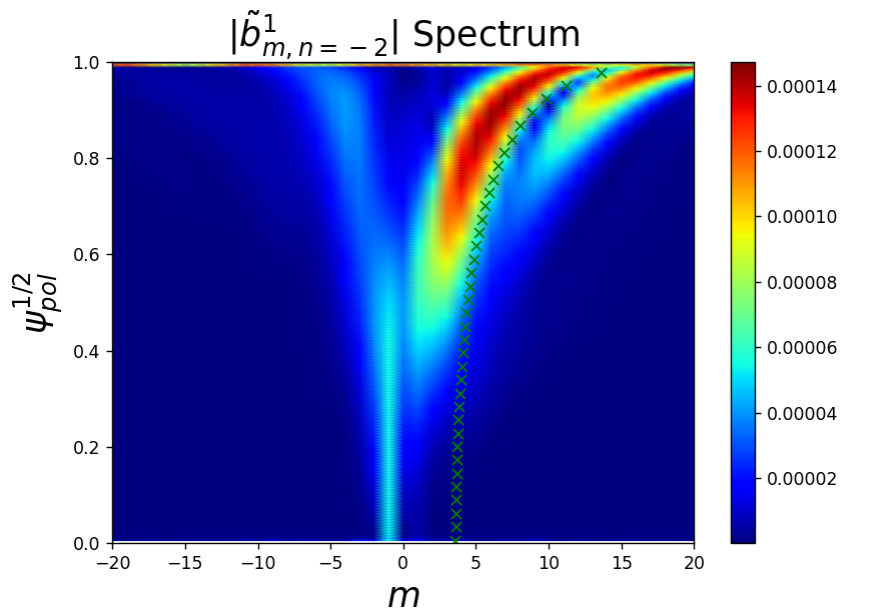
\includegraphics[width=0.7\columnwidth,keepaspectratio]{collab/collab_n=-2_b_sm_nfix_abs.PNG}
    % }
    % \hfill
    % \subcaptionbox{三种线圈共同优化后的结果,在 EAST 73999 Shot 上的 $\tilde{b}^1_{m,n=-2}$ 的相位分布。}{%
    %   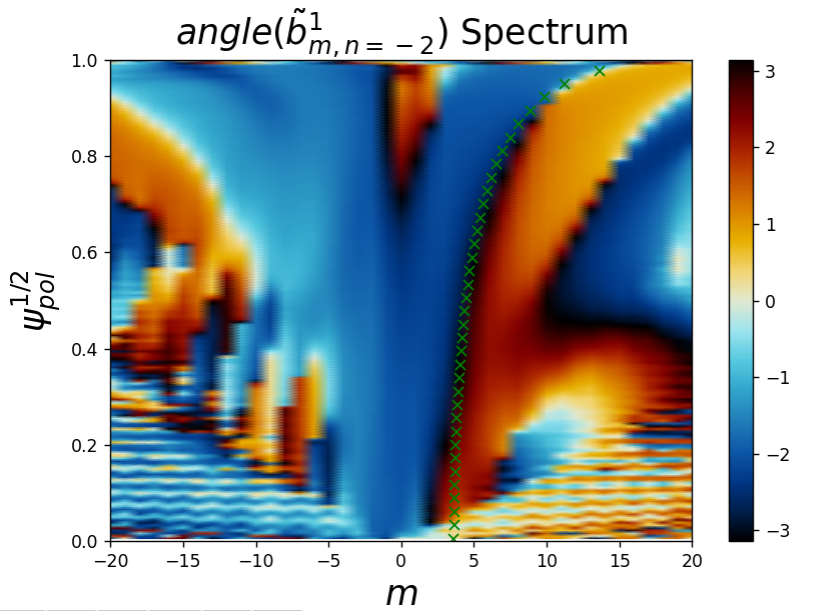
\includegraphics[width=0.47\columnwidth,keepaspectratio]{collab/collab_n=-2_b_sm_nfix_angle.PNG}
    % }%
    \caption{三种线圈共同优化后的结果,在 EAST 73999 Shot 上的 $|\tilde{b}^1_{m,n=-2}|$ 。}
  \end{figure}
  


  
  一开始尝试通过 python 科学计算库 scipy.optimize 函数进行优化得到极值, 但结果中 RMP 线圈的电流值常常在 1 kAt 以下,但高 m 线圈倒是较大,起始以为是陷入了局部极值,随后用了全局随机遍历发现得到的最大值,其对应的磁谱也与上面计算的结果类似,且 RMP 线圈优化得到的电流仍然小于 1 kAt。
  
  

  \begin{figure}[t]
    \centering
    % \subcaptionbox{两种线圈共同优化后的结果,在 EAST 73999 Shot 上的 $\tilde{b}^1_{m,n=-2}$ 的绝对值分布。}{%
      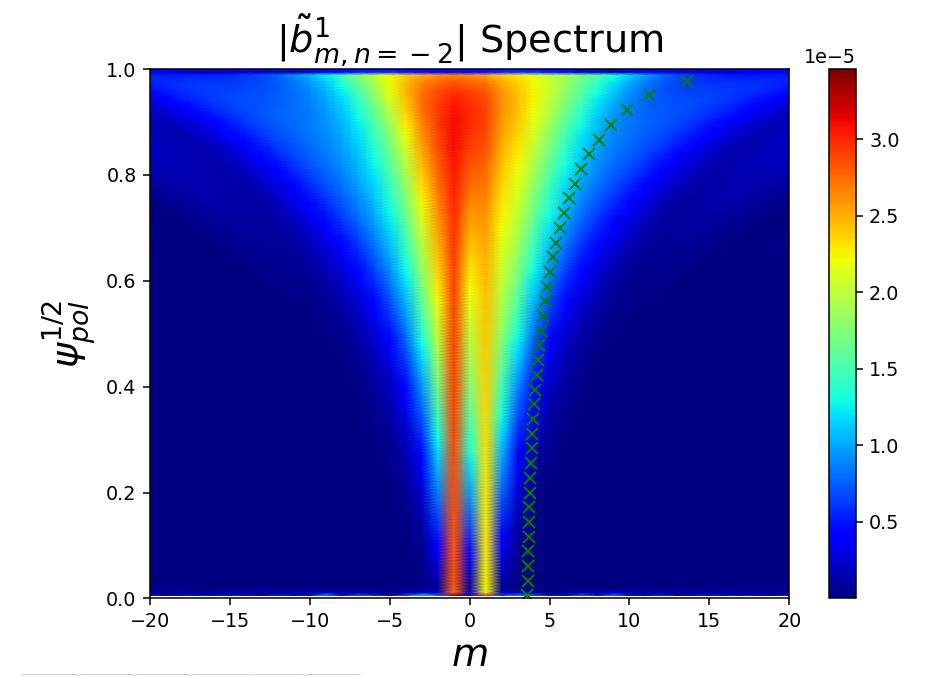
\includegraphics[width=0.7\columnwidth,keepaspectratio]{collab/collab_noHCFs_n=-2_b_sm_nfix_abs.PNG}
    % }%\hfill
    % \subcaptionbox{两种线圈共同优化后的结果,在 EAST 73999 Shot 上的 $\tilde{b}^1_{m,n=-2}$ 的相位分布。}{%
    %   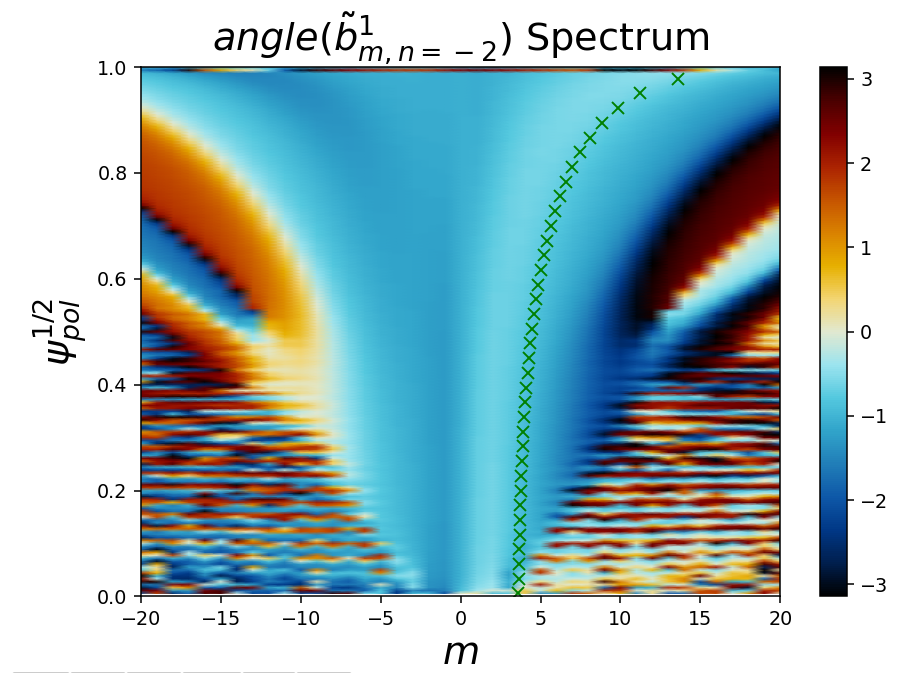
\includegraphics[width=0.47\columnwidth,keepaspectratio]{collab/collab_noHCFs_n=-2_b_sm_nfix_angle.PNG}
    % }%
    \caption{两种线圈共同优化后的结果,在 EAST 73999 Shot 上的 $\tilde{b}^1_{m,n=-2}$ 的绝对值分布。}
  \end{figure}
  
  随机得到的优化值中 RMP 线圈的电流值在 0.1 kAt 以下(高 m 线圈 -9.01486676 kAt),引起了我们进一步的探索。
  
  
  
\begin{figure}[t]
\centering
\label{fig:kAt-FoM}
\subcaptionbox{RMP UP 线圈 kAt 数 - FoM 散点图}{
    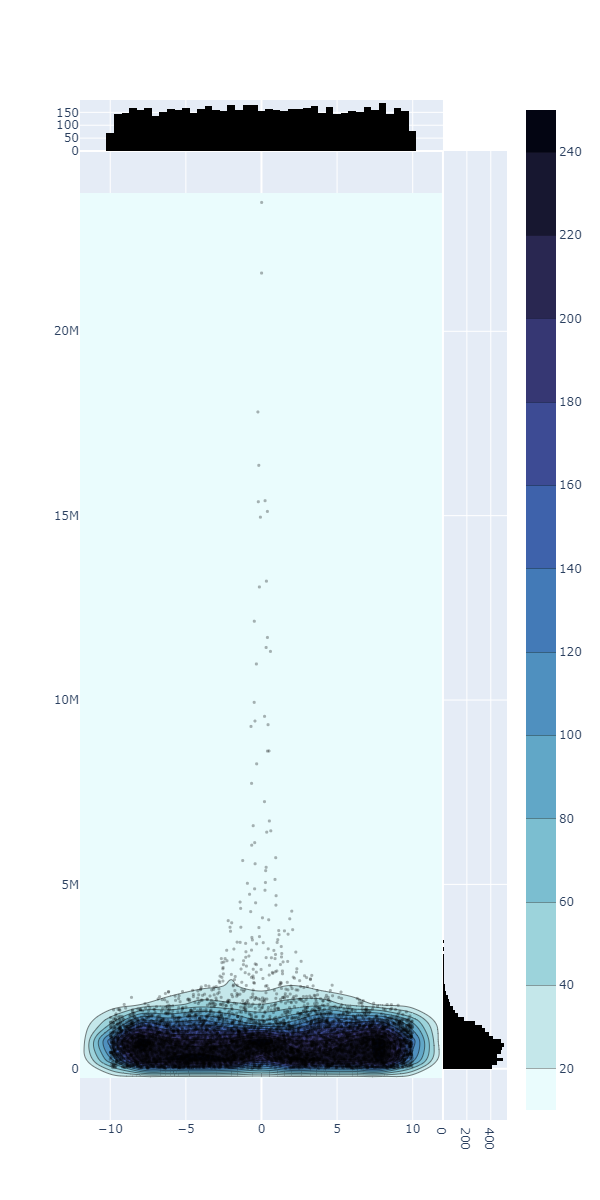
\includegraphics[width=0.32\columnwidth,keepaspectratio]{collab/low_n_UP_FoM.png}
}%\hfill
\subcaptionbox{RMP DOWN 线圈 kAt 数 - FoM 散点图}{
    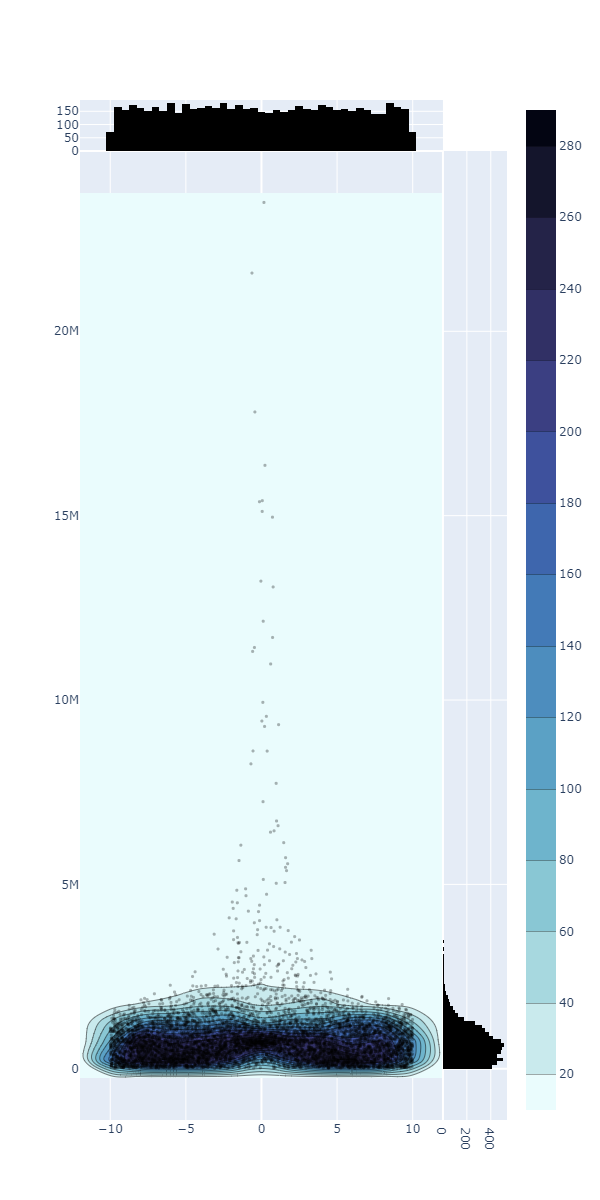
\includegraphics[width=0.32\columnwidth,keepaspectratio]{collab/low_n_DOWN_FoM.png}
}%\hfill
\subcaptionbox{高 m 线圈 kAt 数 - FoM 散点图}{
    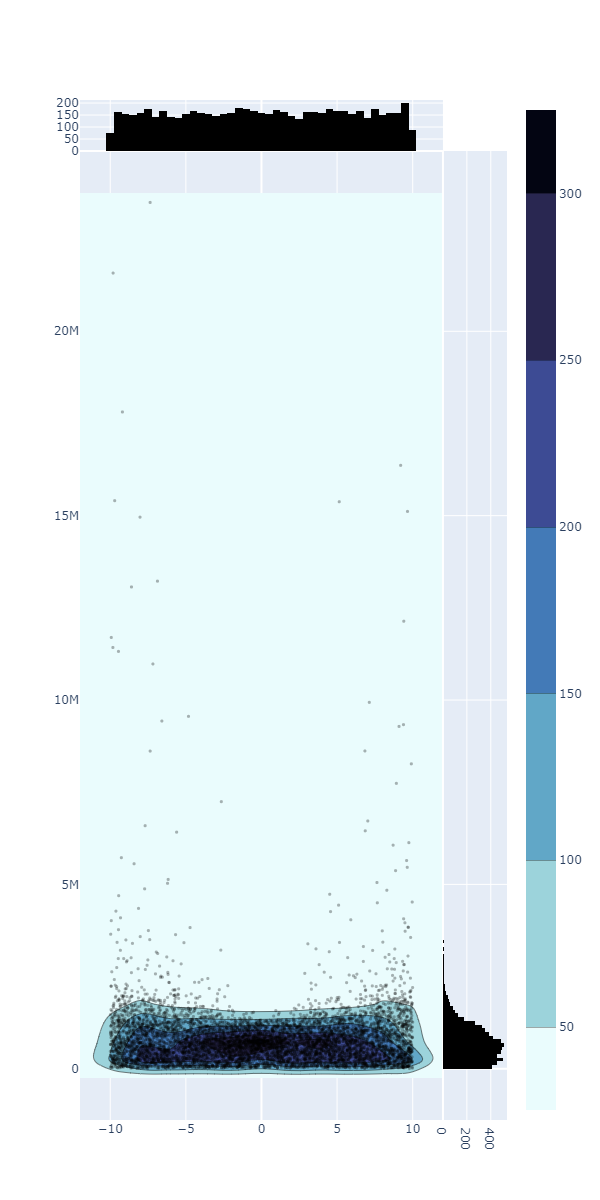
\includegraphics[width=0.32\columnwidth,keepaspectratio]{collab/high_m_FoM.png}
}
\caption{三种线圈电流幅值对品质因子影响的估计}
\end{figure}
  
  

线圈电流幅度对品质因子的影响参见上面几幅图,明显地有着 kAt 数较低 RMP 线圈和较高 kAt 数的高 m 线圈配合有可能产生较高的 FoM 的趋势,。RMP 线圈相位及高 m 线圈旋转角度三者作为坐标轴后作类似上图,未发现明显变化趋势。
  

高 m 线圈的电流幅度的增大会导致高 FoM 时 RMP 线圈的电流幅值容许范围得以增大。
  
  
% \begin{figure}[htbp]
%   \centering%
%       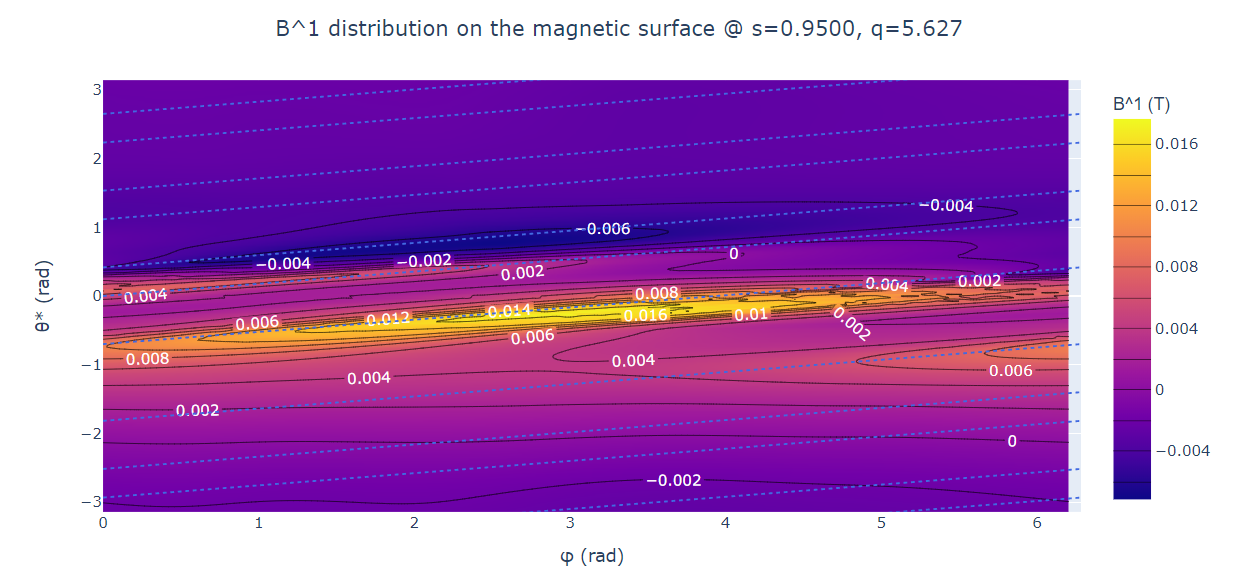
\includegraphics[width=1.0\columnwidth]{hcf/HCFs_uniform.png}
%       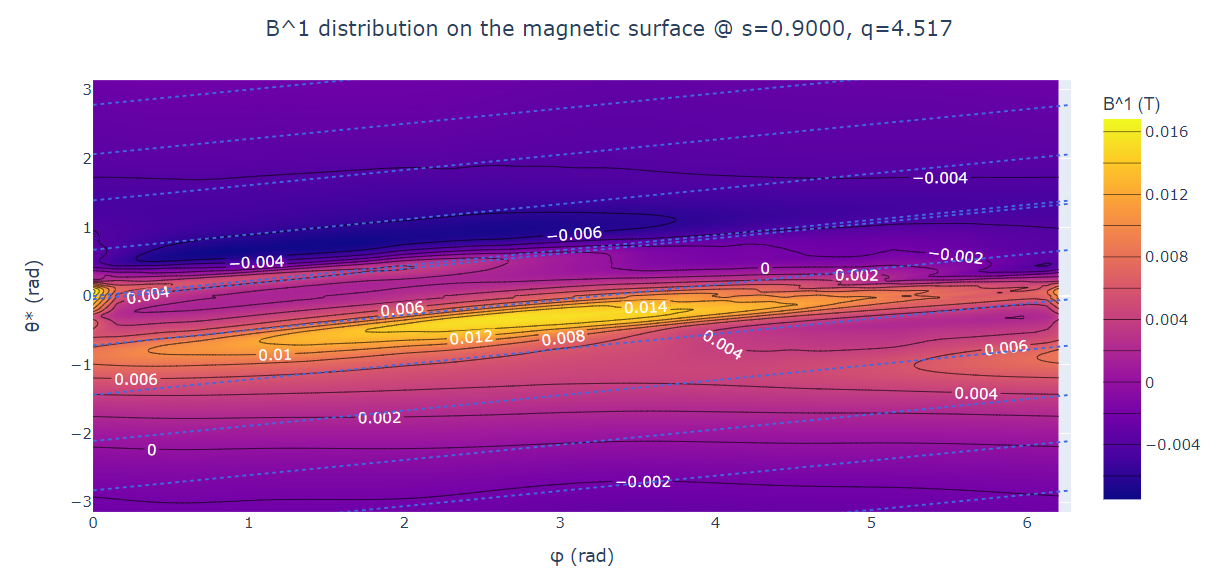
\includegraphics[width=1.0\columnwidth]{collab/collab_n=-2.PNG}
%       \caption{上下图分别为 HCFs 产生的基底磁场和三种扰动场优化后的磁场,各自的 $B^1$ 在磁面上 $s=0.950,0.900$ 的分布。虽然没有控制在一个磁面上,但可见优化后对磁场的影响并不大。}
% \end{figure}
  
  \begin{itemize}
    \item HCFs 产生的磁场太强,忽略它产生的基底磁场重新测试或者增大 RMP、高 m 线圈电流幅值允许范围。
    \item 在 HCFs 的影响下,磁谱脊线并没有向磁面螺旋度对应的曲线靠拢,反倒是原本的脊线最高值变得更高了。 
  \end{itemize}


在上述的问题出现之后,把螺旋电流丝搁置,先研究低 n (RMP) 线圈和高 m 线圈。


\subsection{RMP 线圈与高 $m$ 线圈扰动场共同作用}
随机得到的优化值中 RMP 线圈的电流值在 0.1 kAt 以下(高 m 线圈 -9.01486676 kAt),这意味着和高 m 线圈相耦合的低 n 线圈强度不能过高。该数值实验能帮助我们找到合适的扰动场匹配的大小,比如低 n 线圈(16个)和高 m 线圈(1个)在磁面上的磁通量有数量级的差异,它们应该在磁通量级可比时品质因子有个较好的结果。

\begin{figure}[htbp]
  \centering%
      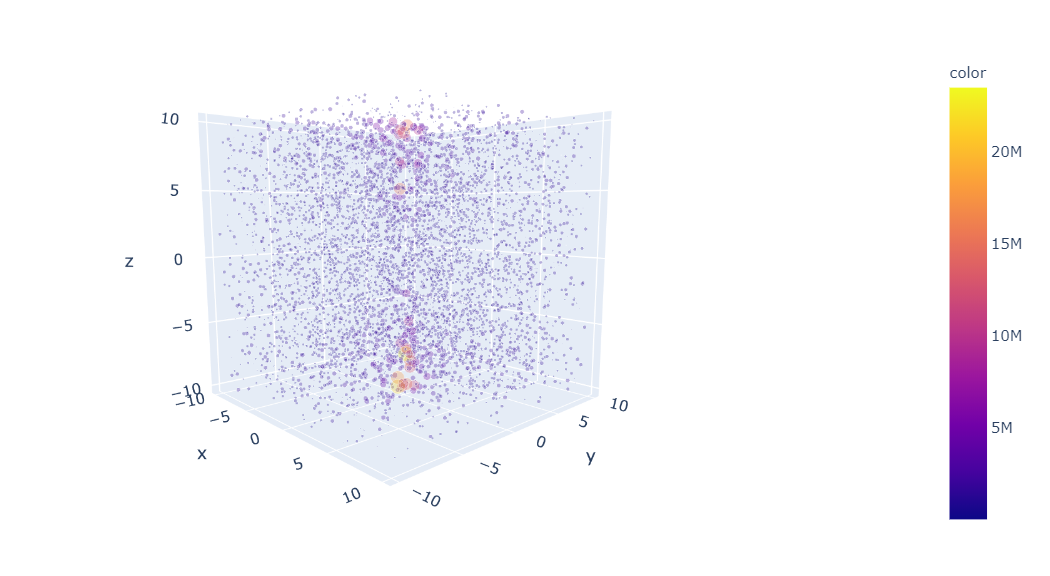
\includegraphics[width=0.5\columnwidth]{collab/Amp_Scatter.png}
      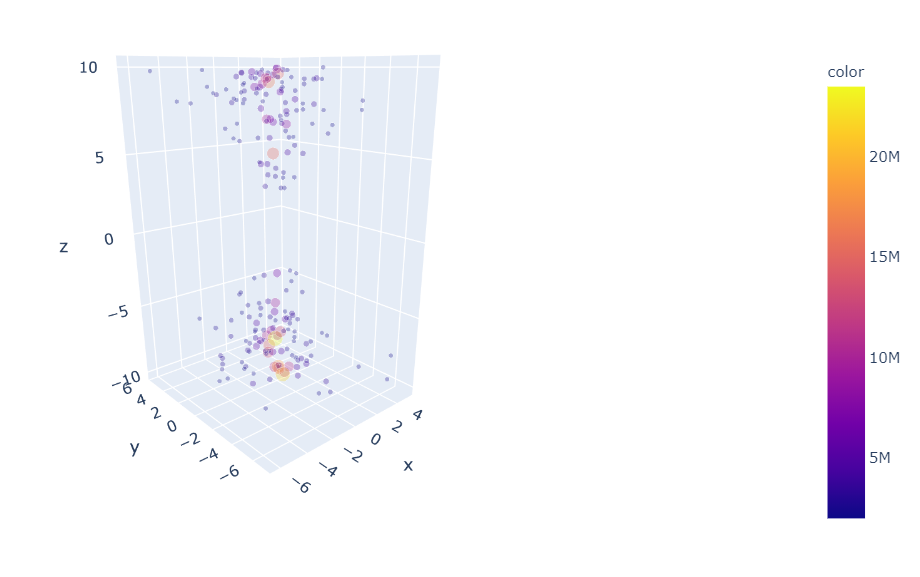
\includegraphics[width=0.45\columnwidth]{collab/Amp_Scatter_FoMthr_2e6.png}
      \caption{左右图均为 RMP 线圈和高 m 线圈进行协同优化后得到的 FoM 分布,marker 的大小和颜色表示 FoM 的大小,坐标轴 XYZ 轴分别为 RMP 线圈上下侧的 电流强度和高 m 线圈的电流强度。右图中过滤去除了 FoM 在 2e6 以下的点。}
\end{figure}

  线圈电流参数对 FoM 的影响参见上面几幅图,明显地有着 kAt 数较低 RMP 线圈和较高 kAt 数的高 m 线圈配合有可能产生较高的 FoM 的趋势。RMP 线圈相位及高 m 线圈旋转角度三者作为坐标轴后作类似上图,未发现明显变化趋势。


  高 m 线圈的电流幅度的增大会导致高 FoM 时 RMP 线圈的电流幅值容许范围得以增大。这告诉我们扰动场的大小要匹配(可以用磁通来衡量扰动场的大小)。


  


  


    
  
% \begin{itemize}
%     \item 对角度 $\varphi$ 这种有界参数,优化问题可以做一个扫描。但一旦引入了各扰动场的相对大小,优化方法可能就必需了。但 ERGOS 只适合串行,考虑将 ERGOS 中计算 Chirikov 径向分布计算等部分单独抽出来。FFT 可以不抽出来,因为线性性和平移性对每个线圈做一次计算就可以了。
% \end{itemize}


    
  

% 以下对三种扰动场仿真模拟细节陈述。

